
\begin{figure}[tp]
  \centering

 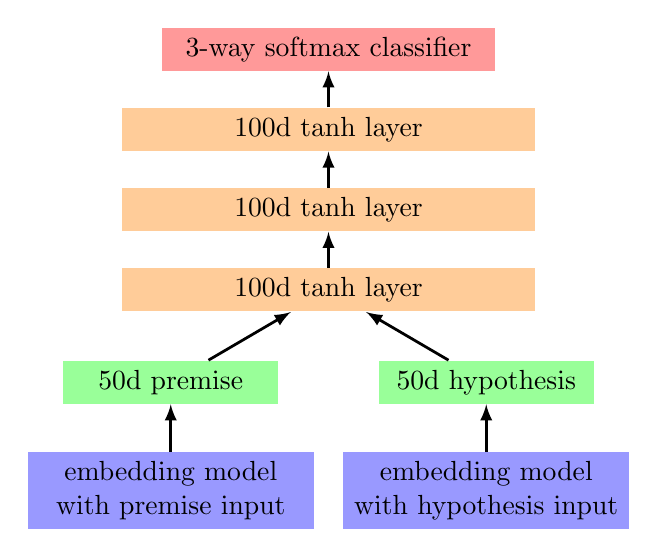
\begin{tikzpicture}
    \def\dx{19pt}
    \def\dy{29pt}

    \tikzstyle{label}=[text width=40mm,align=center]    
    \tikzstyle{softmax}=[fill=red!40,text width=40mm,align=center]
    \tikzstyle{preclass}=[fill=orange!40,text width=50mm,align=center]
    \tikzstyle{e}=[fill=green!40,text width=25mm,align=center]
    \tikzstyle{m}=[fill=blue!40,text width=34mm,align=center]    
    
    \node[softmax]  (softmax) at (0*\dx,6*\dy) {3-way softmax classifier};
    \node[preclass]  (pc3) at (0*\dx,5*\dy) {100d $\tanh$ layer};
    \node[preclass]  (pc2) at (0*\dx,4*\dy) {100d $\tanh$ layer};
    \node[preclass]  (pc1) at (0*\dx,3*\dy) {100d $\tanh$ layer};
    \node[e]  (pe) at (-3*\dx,1.85*\dy) {50d premise};
    \node[e]  (he) at (3*\dx,1.85*\dy) {50d hypothesis};
    \node[m]  (pem) at (-3*\dx,0.5*\dy) {embedding model\\ with premise input};
    \node[m]  (hem) at (3*\dx,0.5*\dy) {embedding model\\ with hypothesis input};    
    
    \pgfsetarrowsend{latex}
    \tikzstyle{fwd} = [draw=black, line width=1pt]

          \draw [fwd] (pc3) -- (softmax);
          \draw [fwd] (pc2) -- (pc3);
          \draw [fwd] (pc1) -- (pc2);
          \draw [fwd] (pe) -- (pc1);
          \draw [fwd] (he) -- (pc1);
          \draw [fwd] (hem) -- (he);
          \draw [fwd] (pem) -- (pe);

  \end{tikzpicture}
	
        \caption{The standard model structure used for entailment evaluation.}
  \label{sample-figure}
\end{figure}